\documentclass{report}
% \documentclass{article}
% Language
\usepackage[T1]{fontenc}
\usepackage[utf8]{inputenc}
\usepackage[english]{babel}

% Page formatting
\usepackage{geometry}
\geometry{a4paper, margin=25mm, includefoot}

% Font, line height, paragraph indentation
% \usepackage{mathptmx} % Times New Roman
\usepackage{newtxtext} % Times New Roman (Modern + Math symbols)
\usepackage[varvw]{newtxmath} % Times New Roman (Modern + Math symbols)

\linespread{1.2}
\setlength{\parindent}{0pt}
% \usepackage{setspace}

% Chapter/section title formatting
\usepackage{titlesec}
\titleformat{\chapter}[display]{\normalfont\Large}{\chaptertitlename\ \thechapter}{0pt}{\huge\bfseries}[\vspace{8pt}\titlerule]
\titlespacing{\chapter}{0cm}{0cm}{0.5cm}

\titleformat{\paragraph}
{\normalfont\normalsize\bfseries}{\theparagraph}{1em}{}
\titlespacing*{\paragraph}
{0pt}{3.25ex plus 1ex minus .2ex}{1.5ex plus .2ex}

% Multi-column TOC
\usepackage{multicol}
% \makeatletter
% \renewcommand{\tableofcontents}[1][\contentsname]{%
%     \chapter*{#1}
%     \begin{small}
%     % \setlength{\columnseprule}{0.5pt}
%     \setlength{\columnsep}{20pt}
%     \begin{multicols}{2}
%         \@starttoc{toc}
%     \end{multicols}
%     \end{small}
% }
% \makeatother

% Used for moving abstract from the center of the page to the top
\usepackage{etoolbox}
\patchcmd{\abstract}{\null\vfil}{}{}{}

% Figures and captions
% \usepackage{caption}
\usepackage{float}
\usepackage{graphicx}
\usepackage{wrapfig}
\usepackage[font=small,labelfont=bf]{caption}
\usepackage[labelformat=simple]{subcaption}
\renewcommand\thesubfigure{(\alph{subfigure})}

\def \FigureAbbreviaition {Fig.}
\newcommand{\figref}[1]{\FigureAbbreviaition\ \ref{#1}}
\newcommand{\tabref}[1]{Table \ref{#1}}
\newcommand{\chapref}[1]{Chapter \ref{#1}}
\newcommand{\algoref}[1]{Algorithm \ref{#1}}

% Figure caption formatting
\AtBeginDocument{%
\captionsetup[figure]{name={\FigureAbbreviaition},aboveskip=10pt,belowskip=-10pt}
\captionsetup[subfigure]{aboveskip=10pt,belowskip=0pt}
\captionsetup[table]{aboveskip=10pt,belowskip=-10pt}
% \captionsetup[subtable]{aboveskip=10pt,belowskip=0pt}
}



% Array
\usepackage{array}
\usepackage{textpos}

% Math and symbols
% \usepackage{amsmath, amssymb, bm} % newtxmath has same defines as amssymb

\usepackage{amsmath}
\newtheorem{problem}{Problem}

% \theoremstyle{remark}

\usepackage{amsmath, bm}
\usepackage{mathtools}
\usepackage{verbatim}
\usepackage{xfrac}
\usepackage{tensor}
\usepackage{interval}
\usepackage{commath} % for \abs, \norm
\usepackage{physics} % for qty(), qty{} etc. (automatic parentheses)

% Custom commands
\usepackage{xstring}
\usepackage{xspace}

\newcommand{\fakecite}[0]{\hl{\textbackslash cite}\xspace}
\renewcommand{\vec}[1]{\ensuremath{\bm{#1}}} % vector [amsmath, bm]

\newcommand{\mat}[1]{\ensuremath{\bm{\mathrm{#1}}}} % matrix [amsmath, bm]
\newcommand{\T}[0]{\top} % transpose ^T
\newcommand{\inv}[0]{\ensuremath{^{-1}}} % inverse ^{-1}
\newcommand{\pinv}[0]{\ensuremath{^{\dagger}}} % pseudo-inverse ^{-1}

\newcommand{\rvec}[1]{\ensuremath{\renewcommand{\arraystretch}{0.6}\begin{bmatrix} #1 \end{bmatrix}}}
\newcommand{\rlist}[1]{\ensuremath{\renewcommand{\arraystretch}{0.6}\begin{Bmatrix} #1 \end{Bmatrix}}}
\newcommand{\cvec}[1]{\ensuremath{\renewcommand{\arraystretch}{1.0}\begin{bmatrix} #1 \end{bmatrix}}}

\newcommand{\twodots}{\mathinner {\ldotp \ldotp}} % .. (two dots)
\renewcommand{\secref}[1]{\hyperref[#1]{\ref*{#1}\ \nameref*{#1}}}
% \newcommand{\tf}[3][T]{\ensuremath{\tensor[^{#2}]{\mat{#1}}{_{#3}}}}
\newcommand{\tf}[3][T]{\ensuremath{{\mat{#1}^{#2}_{#3}}}}

\newcommand{\rot}[3][R]{\ensuremath{{\mat{#1}^{#2}_{#3}}}}

\newcommand{\highlight}[1]{\hl{#1}\xspace}
\newcommand*\of{\qty} % $f\of(x)$
\newcommand{\R}[0]{\mathbb{R}} % real number R

\newcommand{\mvar}[1]{$#1$} % environment for mathematical variable $f(x)$ => \mvar{f(x)}
\newcommand{\robframe}[1]{\mvar{\{\text{#1}\}}}
\newcommand{\inR}[1]{ \in\R^{#1} }
\newcommand{\SE}{ \text{ SE} }

\newcommand{\Csf}{\mathcal{E}_{f,\text{SF}} }
\newcommand{\Chf}{\mathcal{C}_{f,\text{HF}} }

\newcommand{\vsep}{\;} % vector separator
\newcommand{\mfor}{\text{ for }} % for in equation
\newcommand{\mand}{\text{ and }} % and in equation
\newcommand{\mspa}{\qquad} % for in equation


\DeclareMathOperator*{\argmax}{arg\,max}
\DeclareMathOperator*{\argmin}{arg\,min}

% usage: \tf{from}{to} | \tf[T]{from}{to} | \tf[R]{from}{to} | \tf[t]{from}{to} etc.
% \newcommand{\tf}[3][T]{%
%     \IfEqCase{#1}{%
%         {T}{\ensuremath{\tensor[^{#2}]{\mat{#1}}{_{#3}}}}%
%         {R}{\ensuremath{\tensor[^{#2}]{\mat{#1}}{_{#3}}}}%
%         {t}{\ensuremath{\tensor[^{#2}]{\vec{#1}}{_{#3}}}}%
%         {p}{\ensuremath{\tensor[^{#2}]{\vec{#1}}{_{#3}}}}%
%     }[\PackageError{tf}{Undefined option: #1}{}]%
% }%

% Equation spacing
\AtBeginDocument{%
\abovedisplayskip=6pt plus 2pt minus 2pt
\abovedisplayshortskip=6pt plus 2pt minus 2pt
\belowdisplayskip=6pt plus 2pt minus 2pt
\belowdisplayshortskip=6pt plus 2pt minus 2pt
}

% SI units + config and custom units
\usepackage{siunitx}[=v2]
\sisetup{
    per-mode=fraction, fraction-function=\sfrac, % fractions
    % round-mode=figures, round-precision=3, % rounding
    output-exponent-marker=\ensuremath{\mathrm{e}},
    separate-uncertainty=true, multi-part-units=single, % for \SI{2 \pm 0.2}{\rad},
    binary-units=true, % for \byte, \giga etc.
}
\DeclareSIUnit \pixel {px}

% Text highlight (\hl)
\usepackage{soul}

% Enumeration and tables
\usepackage{enumerate}
\usepackage{enumitem}
\usepackage{multirow} 
\usepackage{multicol}
\usepackage{ltablex}
\usepackage{spreadtab}
\usepackage{booktabs}
\usepackage{tabto}
\usepackage{makecell}
\usepackage{diagbox}
\usepackage{tabularx}
\usepackage[export]{adjustbox}


% set max matrix size
\setcounter{MaxMatrixCols}{20}

% \aug for vertical line in matrix
\newcommand\aug{\fboxsep=-\fboxrule\!\!\!\fbox{\strut}\!\!\!}


% Custom tables commands for fixed-column sizes
\newcommand{\PreserveBackslash}[1]{\let\temp=\\#1\let\\=\temp}
\newcolumntype{C}[1]{>{\PreserveBackslash\centering}p{#1}}
\newcolumntype{R}[1]{>{\PreserveBackslash\raggedleft}p{#1}}
\newcolumntype{L}[1]{>{\PreserveBackslash\raggedright}p{#1}}

\setlength\doublerulesep{0.3cm} % when using a double line, make extra space

% Enumeration formatting
\newcommand{\tabitem}{~~\llap{\textbullet}~~}
\newcommand{\sqrbulletsml}{\textcolor{black}{\raisebox{.45ex}{\rule{.6ex}{.6ex}}}}
\newcommand{\sqrbulletmed}{\textcolor{black}{\raisebox{.40ex}{\rule{.7ex}{.7ex}}}}

\renewcommand{\labelitemi}{\sqrbulletmed}
\renewcommand{\labelitemii}{\sqrbulletsml}
\renewcommand{\labelitemiii}{\sqrbulletsml}
\renewcommand{\labelitemiv}{\sqrbulletsml}

% Colors (latexcolor.com)
\usepackage[table]{xcolor}
\definecolor{cerulean}{rgb}{0.0, 0.48, 0.65}
\definecolor{earthyellow}{rgb}{0.88, 0.66, 0.37}
\definecolor{darkmagenta}{rgb}{0.55, 0.0, 0.55}
\definecolor{darkolivegreen}{rgb}{0.33, 0.42, 0.18}
\definecolor{codegray}{gray}{0.9}
\definecolor{gainsboro}{rgb}{0.86, 0.86, 0.86}
\definecolor{cyan}{rgb}{0.0, 1.0, 1.0}

\definecolor{light-yellow}{RGB}{255, 255, 137}
\definecolor{light-blue}{RGB}{148, 201, 233}

\definecolor{tableheader}{gray}{0.9}

\definecolor{metaorange}{rgb}{0.98, 0.54, 0.13} % also known as flame orange

% colored square box
% https://tex.stackexchange.com/questions/201300/inline-boxes-alternative-to-pifonts-non-filled-but-shadowed-box
\newcommand{\sqbox}[1]{\textcolor{#1}{\rule{1.2ex}{1.2ex}}}

% Code snippets
\usepackage{listings}
% \renewcommand{\arraystretch}{1.2}
\renewcommand{\tabcolsep}{0.2cm}
\usepackage{algorithm,algorithmicx,algpseudocode}

% Code snippets formatting
\lstset{
    backgroundcolor=\color{black!5},        % set background color
    basicstyle=\footnotesize\ttfamily,      % basic font setting
    captionpos=b,                           % caption position
    frame=single,                           % draw a frame at the top and bottom of the code block
    framesep=5pt,                           % frame margin
    xleftmargin=5pt,                        % frame margin
    xrightmargin=5pt,                       % frame margin
    tabsize=4,                              % tab space width
    showstringspaces=false,                 % don't mark spaces in strings
    breaklines=true,                        % wrap lines
    commentstyle=\color{darkolivegreen},    % comment color
    keywordstyle=\color{darkmagenta},       % keyword color
    stringstyle=\color{earthyellow},        % string color
    identifierstyle=\color{cerulean},
}

% Custom inline-code command (\code)
%\newcommand{\lstinln}[1]{\colorbox{gainsboro}{\texttt{#1}}}
\newcommand{\code}[1]{%
  \begingroup\setlength{\fboxsep}{2pt}%
  \colorbox{gainsboro}{\texttt{\hspace{2pt}\vphantom{Ay}#1\hspace{2pt}}}%
  \endgroup
}

% package labels
\usepackage{tikz}
\newcommand{\meta}[1]{ \tikz[baseline=(X.base)]\node [draw=metaorange,fill=metaorange,semithick,rectangle,inner sep=2.5pt, rounded corners=2pt] (X) {  \textbf{\textcolor{white}{\textsf{#1}}}}; \hphantom}
\newcommand{\pkg}[1] { \tikz[baseline=(X.base)]\node [draw=blue,fill=blue,semithick,rectangle,inner sep=1.3pt, rounded corners=2pt] (X)             {  \textbf{\textcolor{white}{\textsf{#1}}}}; \hphantom}

% Appendices
\usepackage[toc]{appendix}

% Bibliography and citation
\usepackage[style=numeric, sorting=none]{biblatex}
\usepackage{csquotes}
\DeclareNameAlias{sortname}{family-given}
\DeclareNameAlias{default}{family-given}

% resources
\addbibresource{resources/resources-words.bib}

\addbibresource{resources/resources-appendix.bib}
\addbibresource{resources/resources-introduction.bib}
\addbibresource{resources/resources-modeling.bib}

\addbibresource{resources/resources-problem-1}
\addbibresource{resources/resources-problem-2}
\addbibresource{resources/resources-problem-3}

\addbibresource{resources/resources-sota-problem-1.bib}
\addbibresource{resources/resources-sota-problem-2.bib}
\addbibresource{resources/resources-sota-problem-3.bib}

\addbibresource{resources/resources-system-setup.bib}

% Section cross-referencing
\usepackage{nameref}
\usepackage{hyperref}

\usepackage{bookmark}

% Label counter formatting (e.g. Figure 1 or Figure 2.1)
% In case you want the numbering to start with the chapter number e.g. 1.1 1.2 1.3 for chapter 1 figures, use this instead of the one below
\usepackage{chngcntr} 
\AtBeginDocument{%
    \counterwithin{figure}{chapter}
    \counterwithin{table}{chapter}
    \counterwithin{equation}{chapter}
    \counterwithin{lstlisting}{chapter}
}

\usepackage{tcolorbox}
\tcbuselibrary{theorems}

% In case you want the numbering to continue between chapters e.g. 1 2 3 4 5, use this instead of the one above
% \usepackage{chngcntr} 
% \AtBeginDocument{%
%     \counterwithout{figure}{chapter}
%     \counterwithout{table}{chapter}
%     \counterwithout{equation}{chapter}
%     \counterwithout{lstlisting}{chapter}
% }

% Glossaries and acronyms
% must be loaded last + no empty includes in main document.
\usepackage[automake, acronym, nogroupskip, nonumberlist]{glossaries}
\usepackage{glossary-mcols}
\setglossarysection{section}

% command for dual entries
% \newdualentry[<options>]{<label>}{<abbrv>}{<long>}{<description>}
% https://tex.stackexchange.com/a/368666
\newcommand*{\newdualentry}[5][]{%
  \newglossaryentry{main-#2}{%
    name={#4 (\glslink{#2}{#3})},%
    text={#3\glsadd{#2}},%
    description={{#5}},%
    #1%
  }%
  \newglossaryentry{#2}{%
    type=\acronymtype,%
    first={\glslink{main-#2}{#4 (#3)}},%
    name={#3\glsadd{main-#2}},%
    description={\glslink{main-#2}{#4}},%
    plural={#2s},%
    firstplural={\glsentrydesc{#2}s (\glsentryplural{#2})}
  }%
}

% setup and load glossaries
\makeglossaries
\loadglsentries{glossary}

% only hyperlink first-time glossary entries
% \renewcommand*{\glslinkcheckfirsthyperhook}{%
%   \ifglsused{\glslabel}%
%   {%
%     \setkeys{glslink}{hyper=false}%
%   }%
%   {}%
% }

% generate word count text file wc.tex
\immediate\write18{bash wc.sh}

\begin{document}

% title page

\begin{titlepage}
    \begin{center}
   
        \vspace{0.5cm}
        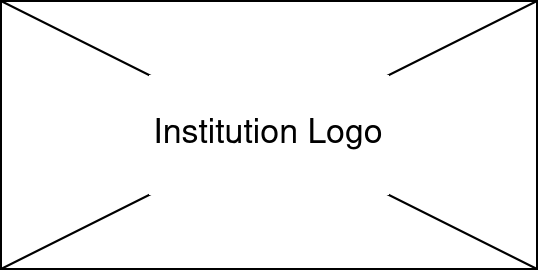
\includegraphics[width=5cm]{img/institution-logo.png}
        \vspace{1cm}
        
        {\LARGE Title \par}


        \vspace{1cm}
        \textbf{Master Thesis}
        \vspace{0.5cm}
       
        written by
       
        \vspace{0.5cm}
        
        \begin{tabular}[t]{c@{\extracolsep{4em}}}
        \textbf{Name Surname}\\
        example@mail.com\\
        \end{tabular}
        
        \vspace{2.0cm}
        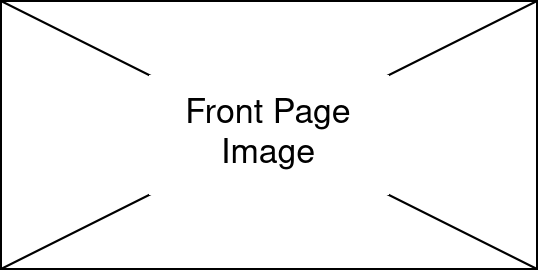
\includegraphics[width=0.5\textwidth]{img/front-page-image.png}
        \vspace{2.0cm}
        
        \begin{center}
        The code for this project is available at\\
        \url{https://some-github-url.com}
        \end{center}
        
        \vfill
        
        \textbf{Institution}\\  
        Faculty\\
        
        \vspace{0.5cm}
        
        Word Count : 17157
 \\
        \today
            
   \end{center}
\end{titlepage}

% preface
% \input{sections/0-preface}

% roman numbering for abstract, TOC, glossary etc.
\pagenumbering{roman}

% abstract
\clearpage
\begin{abstract}
\setlength{\parindent}{0pt}
\normalsize

\noindent Some abstract text explaining the goal, methods and conclusion of the project. \\

\end{abstract}

% table of contents
\clearpage
\tableofcontents

% workload distribution
\clearpage

\section*{Acknowledgements}

Crafting an acknowledgement paragraph in a thesis is a heartfelt opportunity to express gratitude and recognition for the individuals and institutions that have contributed to the completion of the work. It's a chance to acknowledge the guidance, support, and inspiration received throughout the research journey. In this paragraph, one can extend appreciation to mentors, advisors, professors, and peers whose expertise and encouragement shaped the thesis. Personal gratitude to family and friends who provided emotional support during the challenging phases of research is also appropriate. Additionally, acknowledging funding sources, research facilities, and organizations that played a role in the project's success underscores the collaborative nature of academic pursuits. An acknowledgement paragraph, while concise, carries sincere sentiments that honor the shared effort and collaboration that culminated in the completion of the thesis.

\addcontentsline{toc}{section}{Acknowledgments}

% glossary & acronyms
\clearpage
\addcontentsline{toc}{section}{Acronyms and Terms}
\printglossary[type=acronym, title=Acronyms, style=mcolindex]
\printglossary[type=main, title=Terms]

% main document
\clearpage
\pagenumbering{arabic}
\glsresetall

\pagebreak
\chapter{Example section}\label{ch:example}

This document demonstrate the use of figures, references, SI units, glossary, math notation, lists, and otherwise relevant formatting specifications. Paragraphs are typically separated using \texttt{\textbackslash medskip}.\medskip

\begin{figure}[H]
    \centering
    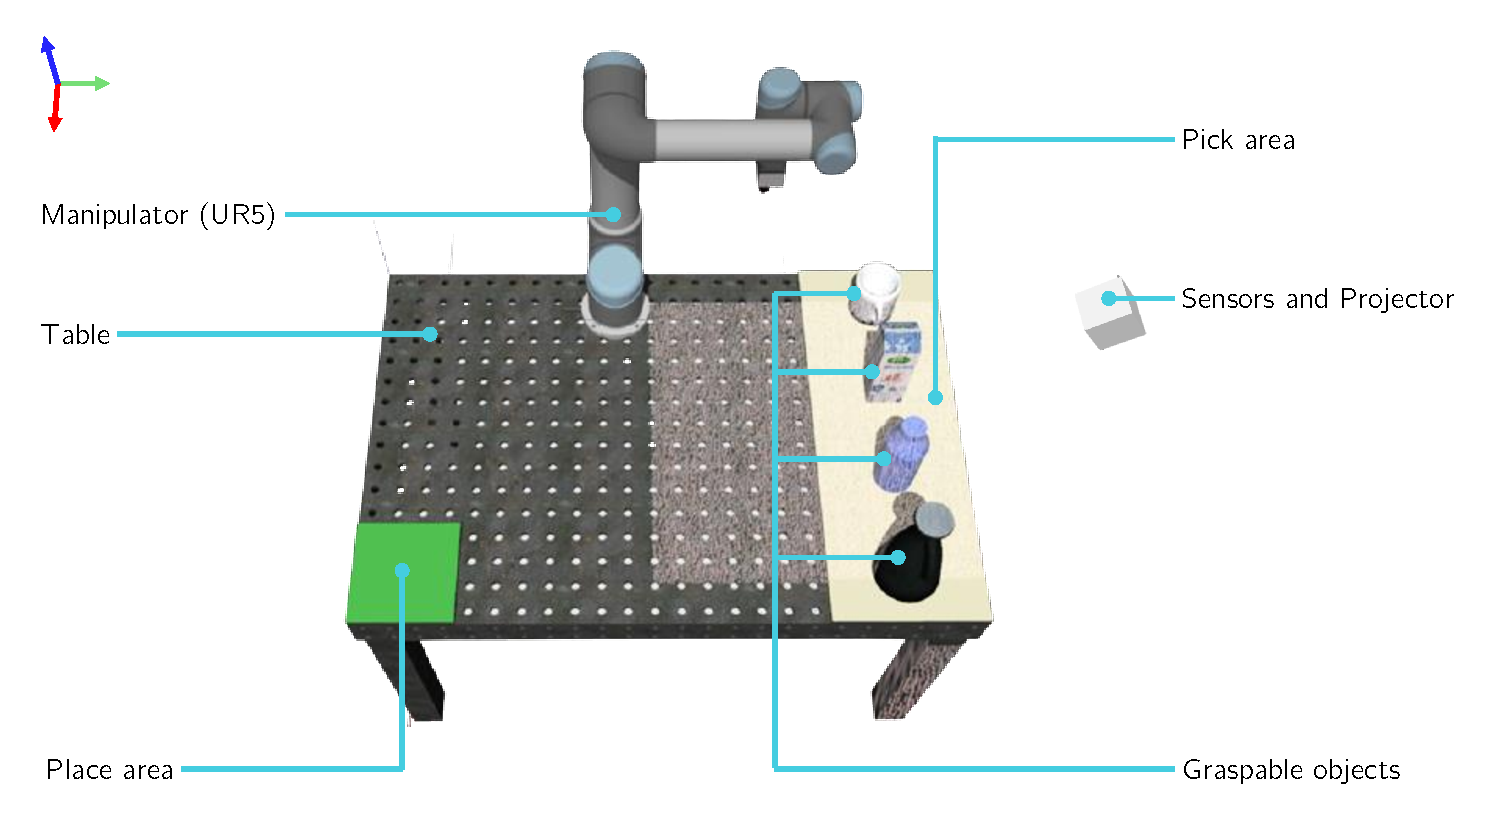
\includegraphics[width=.6\linewidth]{chapters/example/fig/figure.pdf}
    \caption{An example image using \acrlong{acronym-label}.}
    \label{fig:example-figure}
\end{figure}

To exemplify math notation, consider the mapping between the joint configuration of a robot
%
\begin{equation}
    \vec{q} = \rvec{q_1 & q_2 & \dots & q_n}\T,
    \label{eq:jnt-config}
\end{equation}

and \gls{glossary-label}, given as a homogeneous transformation
%
\begin{equation}
    \renewcommand{\arraystretch}{1.2}
    \tf{A}{B} = \begin{bmatrix}
        \tf[R]{A}{B}         & \tf[t]{A}{B} \\
        \vec{0}^{1 \times 3} & 1 
    \end{bmatrix},
\end{equation}

where \tf[R]{A}{B} and \tf[t]{A}{B} is the rotation and translation, respectively, from frame $\{A\}$ to frame $\{B\}$, denoted using a homogeneous transformation matrix $\mat{T}(\vec{q}) \in \mathbb{R}^{4 \times 4}$ as a function of the joint configuration in \eqref{eq:jnt-config}, as described in \cite{robotics-book}.\medskip

Complex table/figure hybrids with aligned captions and functioning labels can be implemented using \texttt{minipage}, as shown in \tabref{tab:example-table} and \figref{fig:example-plot}. Use \fakecite as a placeholder for citations.

\begin{center}
    \renewcommand{\arraystretch}{1.2}
    \begin{minipage}{.4\linewidth}
        \vspace{-10pt}
        \centering
        \begin{tabular}{|l|c|c|c|}
        \hline
        \diagbox[width=5.5em, font=\footnotesize\bfseries]{Method}{Pose} & 1 & 2 & 3 \\ \hline
        Linear    & \SI{18.97}{\second} & \SI{20.35}{\second} & \SI{22.85}{\second} \\ \hline
        Parabolic & \SI{13.66}{\second} & \SI{14.93}{\second} & \SI{17.33}{\second} \\ \hline
        \end{tabular}%
    \end{minipage}%
    \hfill%
    \begin{minipage}{.55\linewidth}
        \vspace{0pt}
        \centering
        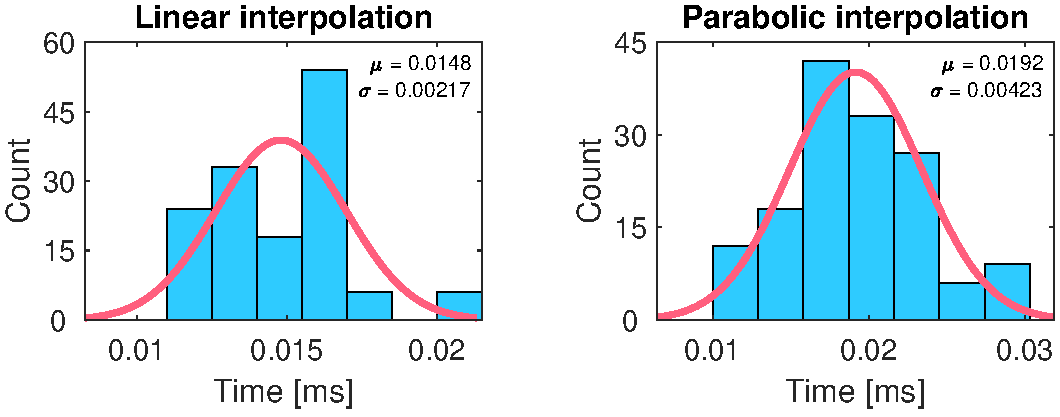
\includegraphics[width=.95\textwidth]{chapters/example/fig/plot.pdf}
    \end{minipage}%
    %    
    \vspace{15pt}
    %
    \begin{minipage}[t]{.4\linewidth}
        \vspace{0pt}
        \captionsetup{type=table}
        \captionof{table}{Trajectory durations of the interpolation-based trajectory generation methods.}
        \label{tab:example-table}
    \end{minipage}%
    \hfill%
    \begin{minipage}[t]{.55\linewidth}
        \vspace{0pt}
        \captionsetup{type=figure}
        \captionof{figure}{Average planning time for each of the interpolation-based trajectory generation methods.}
        \label{fig:example-plot}
    \end{minipage}%
\end{center}

For numbers, units and ranges, the \texttt{siunitx} package is used, which allows to express a number \num{10}, a range of \SIrange{5}{6}{\second}, or a SI unit of \SI{5.73 \pm 1.09}{\second}. Inline row-vectors (with the transpose symbol) can be written as $\vec{a} = \rvec{\vec{a}_p & \vec{a}_o}\T$, where as parentheses can be automatically written using $\qty(a, b)$ or $\qty{\frac{a}{b}, c}$. Also, shorthands for \mat{A}\inv, \mat{A}\pinv and \mat{A}\T.\medskip

\glsresetall

\pagebreak
\chapter{Introduction}\label{ch:intro}

\section{Context}\label{sec:intro-context}

The contextual section within a thesis introduction serves as a bridge between the general knowledge of the field and the specific focus of your research. This section provides readers with essential background information that helps them understand the broader context within which your study operates. To write an effective contextual section, begin by outlining the foundational concepts, theories, and existing research relevant to your topic. Highlight key developments, debates, and gaps in the literature that your research aims to address. You can also mention any real-world implications or applications of your work. By carefully weaving together the established knowledge in the field and your research's niche, the contextual section sets the stage for the reader, preparing them to appreciate the significance and uniqueness of your study. Balancing conciseness with clarity, the section should smoothly transition from the general to the specific, ensuring that your research's importance is clearly conveyed within the broader academic landscape.

\section{Problem Description}\label{sec:intro-problem-description}
Writing a problem description in a thesis involves articulating the central challenge or question that your research aims to address. It is a critical section that sets the context for your work, highlighting its significance and relevance. To effectively write a problem description, start by clearly defining the problem, outlining its scope, and emphasizing its real-world implications. Provide background information to help readers understand the context and the gaps in existing knowledge or practices that your research seeks to fill. Use clear and concise language to convey the problem's complexity while avoiding unnecessary jargon. Consider incorporating relevant statistics, anecdotes, or examples to illustrate the problem's impact. Additionally, acknowledge existing research and solutions related to the problem, emphasizing the unique perspective or approach your study brings. Ultimately, a well-crafted problem description should engage readers' interest and lay the foundation for the subsequent sections of your thesis. \medskip

The problem can ideally be decomposed into some number of sub-problems, that here can be presented. These can later have their own chapters, literature review etc.
% and end effector pose est
\section{Thesis Overview}\label{sec:intro-thesis-overview}

Composing a thesis overview is a foundational step in guiding readers through the content and scope of your research. This succinct yet informative section serves as a roadmap, providing readers with a clear understanding of the purpose, structure, and key elements of your thesis. Begin by introducing the broader research topic and its significance, highlighting the gap in existing knowledge or the problem you aim to address. Subsequently, briefly outline the main research questions, hypotheses, or objectives that your thesis seeks to answer or achieve. Mention the methodology or approach you adopted and provide a glimpse of the primary findings or outcomes. Additionally, touch upon the organization of the subsequent chapters, delineating how each chapter contributes to the overall narrative. The overview should strike a balance between providing enough context for readers to engage with your work and maintaining conciseness to maintain their interest. In essence, a well-crafted thesis overview offers a panoramic view of your research journey, setting the stage for a coherent and engaging exploration of your thesis.

\pagebreak
\chapter{Problem 1} \label{ch:problem1}


\section{Introduction} \label{sec:problem1-introduction}
Here we write the introduction for problem 1.


\section{Related Work} \label{sec:problem1-related-work}

Here we cite the related work by \texttt{\textbackslash cite\{source-label\}} like this \cite{example-article}

\pagebreak
\chapter{Problem 2} \label{ch:problem2}

\pagebreak
\chapter{Discussion} \label{ch:discussion}

\pagebreak
\chapter{Conclusion} \label{ch:conclusion}

% bibliography
\pagebreak
% \printbibliography[heading=bibintoc]
\begin{multicols}{2}[\printbibheading]
\printbibliography[heading=none]
\end{multicols}

\appendix
\chapter{Appendix of Problem 1}\label{app:shadow-dexterous-hand-technical-specifications}

\chapter{Appendix of Problem 2}\label{app:tactile-perception-simulated-electrode-activations}

\chapter{Appendix of Problem 3}\label{app:pose-estimation-weight-convergence}


\end{document}